\chapter{Arbeitsweise}
\label{chap:arbeitsweise}
%1.Unterkapitel
\section{Tensoren}
\label{sec:tensoren}
\printsubchapterauthor{\authorNiklas}

\subsection{Mathematische Definition}
\label{sec:mathematischeDefinition}
\begin{center}
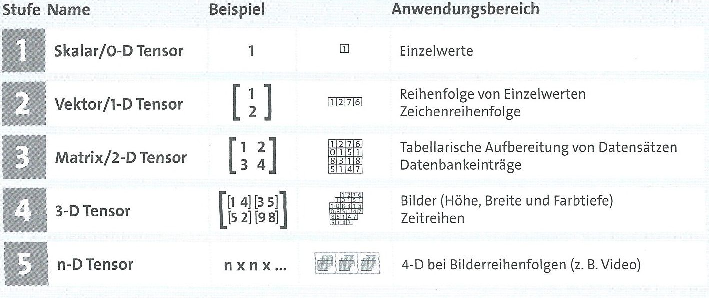
\includegraphics[width=.6\textwidth]{../abbildungen/5-9.pdf}
	\captionof{figure}{Verschiedene Tensoren und ihre Anwendungsbereiche (vgl.\citep{DeepLearning}, S.136)}
	\label{fig:tensoren}
\end{center}

Ein Tensor ist eine Bezeichnung für ein n-dimensionales Feld. In der Abbildung \ref{fig:tensoren} sind unterschiedliche Dimensionen von Feldern dargestellt. Tensoren können von einem einfachen Skalar bis zu merhdimensionalen Feldern reichen.\citep{Einfuehrung}

\subsection{Tensoren in TensorFlow}
\label{sec:tensorenInTensorflow}
In TensorFlow hingegen werden die Daten, die durch den Graphen fließen Tensoren genannt. Da diese Daten wie die Tensoren in der Mathematik verschiedene Dimensionen annehmen können, wie zum Beispiel einfache Zahlenwerte oder dreidimensionale Felder eines Bildes, basiert der Begriff auf dem mathematischen Begriff. 

Tensoren besitzen in TensorFlow die Attribute Name, Shape und Datentyp. Diese Attribute können bei der Initialisierung gesetzt werden oder sie werden von TensorFlow automatisch hinzugefügt. TensorFlow unterstützt sehr viele Datentypen. Diese sind in der Tabelle \ref{fig:datentypenTabelle} zu sehen.\\
\begin{center}
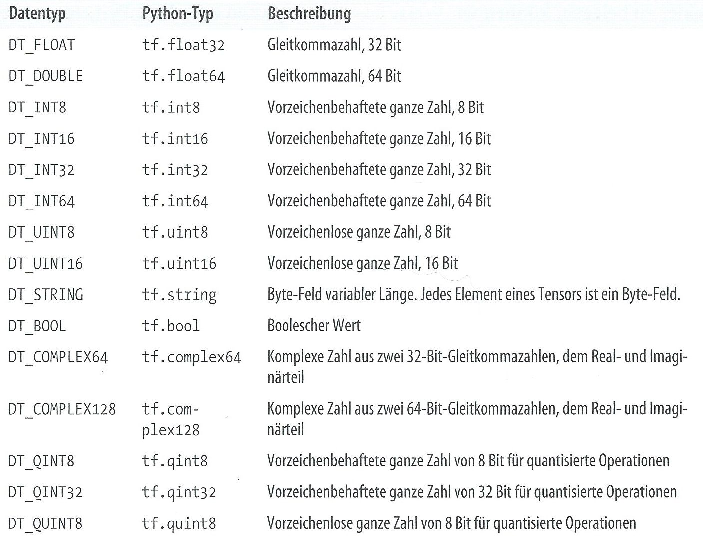
\includegraphics[width=.6\textwidth]{../abbildungen/Tabelle3-2.pdf}
	\captionof{figure}{Tabelle der TensorFlow Datentypen (vgl.\citep{Einfuehrung}, S.33)}
	\label{fig:datentypenTabelle}
\end{center}
Bei der Verwendung von unterschiedlichen Datentypen ist es wichtig eine Typcast zu verwenden, da sonst eine Ausnahme geworfen wird. Das Attribute Shape gibt an, ob es sich bei diesem Tensor um eine Skalar, einen Vektor, eine Matrix oder ein mehrdimensionales Feld handelt. Wenn das Shape-Attribut zum Beispiel die Werte (2, 3) besitzt, kann es für die Matrix $\mathit{[[1, 2, 3], [4, 5, 6]]}$ stehen, da diese aus zwei Zeilen und 3 Spalten besteht.\\
Da die Eingabeschicht eines Neuronalen Netzes die Eingabedaten anders verarbeitet als die inneren Schichten, besitzt TensorFlow drei unterschiedliche Arten von Tensoren. Für die Eingabeschicht werden die sogenannten \textbf{Platzhalter} genutzt. Bei der Initialisierung muss nur der Datentyp übergeben werden. Die Daten werden bei der Ausführung einer Session über ein 'feed-dictionary'  an die Eingabeschicht übergeben. In den inneren Schichten werden meistens \textbf{Variablen} verwendet, da es möglich sein muss, die Gewichte nach einem Durchlauf korrigieren zu können. Zur Initialisierung der Variablen muss ein Startwert angegeben werden. Außerdem ist es möglich \textbf{Konstanten} zu verwenden. Wie bei üblichen Konstanten können die Werte von Konstanten in TensorFlow nicht verändert werden, deswegen ist es nötig darauf zu achten, wo genau diese verwendet werden.
Bei der Ausführung einer Operation entstehen ebenfalls Objekte von Tensoren, deshalb müssen Operationen einer Variablen zugeordnet werden. Hier ist mit einer Variablen jedoch nicht das gleiche gemeint, wie im Vorherigen beschrieben sondern nur eine einfache Zuordnung. In dem folgendem Beispiel entsteht aus der Addition der beiden Konstanten a und b eine neue Variable c.
\begin{center}
a = tf.constant(5)\\ b = tf.constant(4)\\ c = tf.add(a, b)    
\end{center}

%2.Unterkapitel
\section{Operationen}
\label{sec:operationen}
\printsubchapterauthor{\authorMarco}
TensorFlow bietet verschiedenste Operationen zum Arbeiten mit Tensoren an. Diese können in verschiedene Gruppen untergliedert werden. Die ersten beschäftigen sich mit dem Erstellen von Graphen und Tensoren. Beispiele dafür sind tf.constant oder tf.zeros, welche einen konstanten Tensor oder einen Tensor mit Nullen erstellen. Weitere Operationen beinhalten mathematische Funktionen. Dabei sind sowohl Grundrechenarten als auch Exponentialrechnungen, trigonometrische Funktionen, Vergleiche, Rundungen und mehr vertreten. Weiterhin gibt es Operationen zum Verändern von Strings, Bildern und anderen nicht rein numerischen Tensoren. Diese können Bilder erhellen, den Kontrast ändern oder Bilder spiegeln. Dazu gibt es noch mehr Operationen, die verschiedene Inputs bearbeiten können. Dazu zählen auch Konsoleneingaben durch den Nutzer.

%3.Unterkapitel
\section{Graphen}
\label{sec:graphen}
\printsubchapterauthor{\authorNiklas}
\subsection{Aufbau}
\label{sec:graphenAufbau}
Wie schon in Kapitel \ref{sec:allgemeines} erwähnt, arbeitet TensorFlow auf einem Datenflussgraphen. Dabei handelt es sich um ein gerichtetes Diagramm, das ein mathematisches Problem darstellt. Diese Datenflussgraphen bestehen aus Tensoren \ref{sec:tensoren} und Operationen \ref{sec:operationen}, die miteinander verbunden sind. Dabei werden die Operationen als Knoten und die Tensoren als Kanten dargestellt. Durch eine Aneinanderreihung von unterschiedlichen Operationen, mit den dazugehörigen Tensoren als Werte, entsteht ein Datenflussgraph. Dieser wird als mathematische Grundlage für ein Neuronales Netz oder für einfache Berechnungen genutzt.

\subsection{Funktionsweise}
\label{sec:graphenFunktionsweise}
\begin{center}
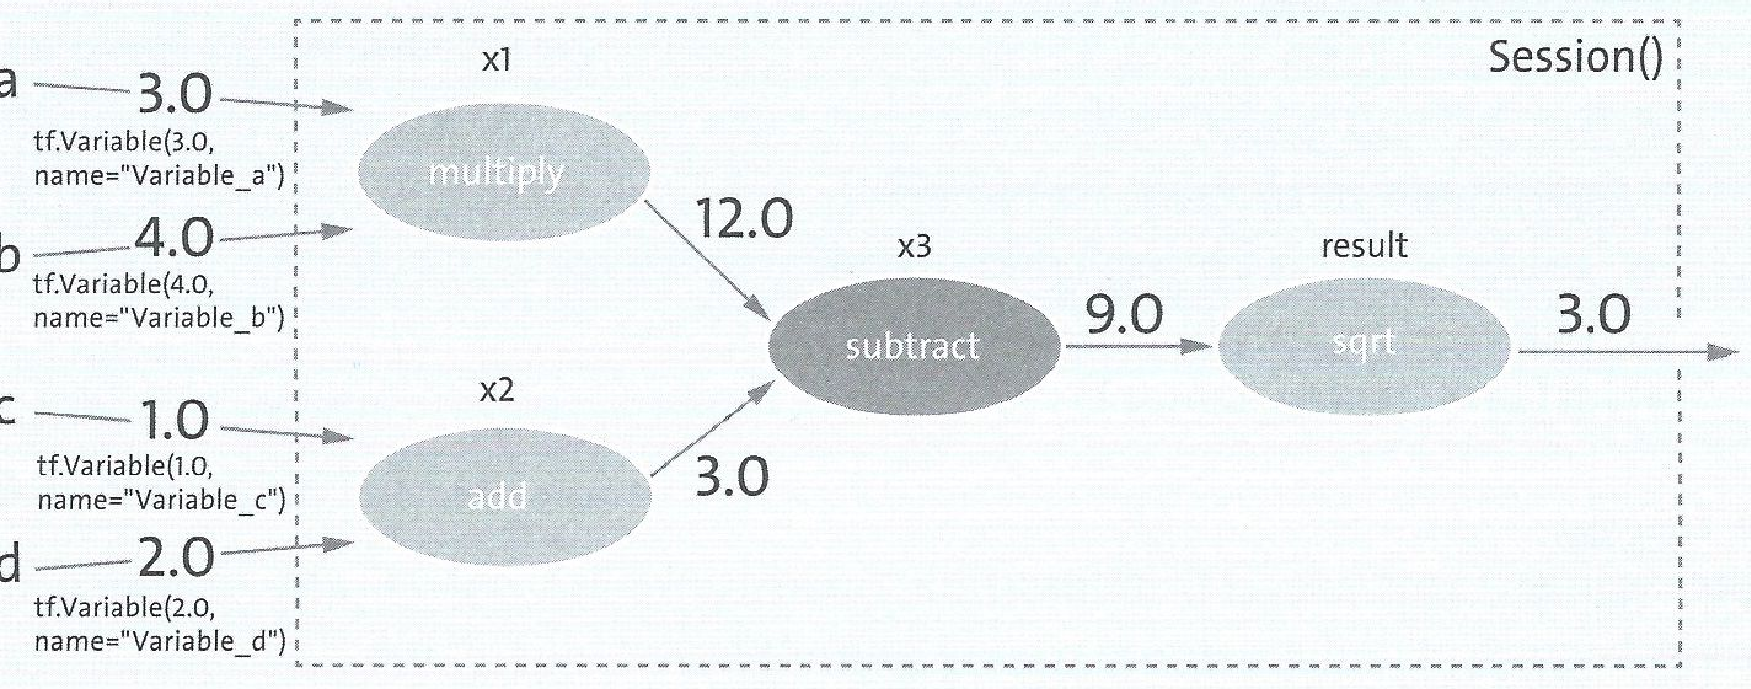
\includegraphics[width=.6\textwidth]{../abbildungen/5-11.pdf}
	\captionof{figure}{Beispiel eines Datenflussgraphs (vgl.\citep{DeepLearning}, S.142)}
	\label{fig:beispielGraph}
\end{center}
Die Abbildung \ref{fig:beispielGraph} zeigt eine einfache Berechnung als Datenflussgraphen, um den Ablauf zu verdeutlichen. Der Code dieses Graphen ist im Anhang \ref{sec:codeBeispielGraph} zu finden. Die Berechnung eines Graphen kann nur in einem \textit{tf.Session()}-Block ausgeführt werden. Am Anfang dieses Blocks wird zusätzlich eine \textit{tf.Session()} Variable angelegt. Dies wird durch den Ausdruck \textit{with tf.Session() as sess} realisiert. Das \textit{Session()}-Objekt wird später benötigt, um diese zu starten. Bevor die \textit{Session} gestartet wird, werden die Konstanten, oder auch Tensoren, a, b, c und d erstellt und ein Wert zugewiesen. Die letzte Operation wurde dem Tensor \textit{result} in der Form \textit{result = tf.sqrt(x3, "Wurzel")} zugewiesen. Für den Start muss der Operation der Tensor übergeben werden, der berechnet werden soll. Diese Operation muss zusätzlich einer Variablen übergeben werden, damit der Wert weiter verwendet werden kann. In diesem Fall sieht die Funktion wie folgt aus: \textit{res = sess.run(result)}. Über die Variable \textit{res} kann nun das Ergebnis ausgegeben werden. In diesen Beispiel wurden nur die TensorFlow-Konstanten verwendet. Auf die Benutzung von Variablen und Platzhaltern wird in dem Kapitel \ref{sec:ablauf} weiter eingegangen.

Durch die Verwendung von Graphen ist es möglich einzelne Operationen ohne große Umstände austauschen  und die jeweiligen Auswirkungen direkt testen zu können. Ein weiterer großer Vorteil des Datenflussgraphen ist die Festellung der Abhängigkeiten zwischen den einzelnen Berechnungen des Graphen. Durch diese Abhängigkeiten ist es möglich den Graphen in Untergraphen zu unterteilen und auf unterschiedlichen Recheneinheiten ausführen zu lassen. 

\begin{center}
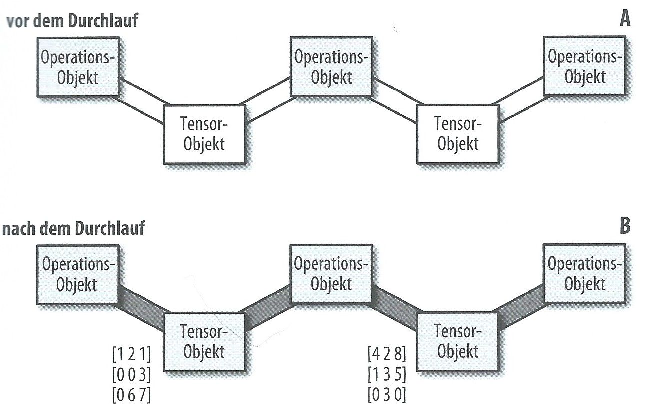
\includegraphics[width=.6\textwidth]{../abbildungen/3-4.pdf}
	\captionof{figure}{Datenflussgraph vor und nach eines Durchlaufs (vgl.\citep{Einfuehrung}, S.31)}
	\label{fig:vorUndNachSession}
\end{center}
Vor der Ausführung eines \textit{Session}-Blocks enthalten die Variablen nur Referenzen der Objekte, die für die Berechnung verwendet werden sollen und keine konkreten Daten. Dies ändert sich mit dem Start der Ausführung und dem Durchlaufen der Operationen. Wie in der Abbildung \ref{fig:vorUndNachSession} zu sehen ist werden die Referenzen der Tensor-Objekte in A durch Tensor-Objekt-Instanzen ersetzt.

\subsection{Darstellung von Operationen}
\label{sec:darstellungOperationen}
Im Kapitel \ref{sec:operationen} wurde im Allgemeinen auf die Operationen in TensorFlow eingegangen. Dies wird nun noch für die Darstellung vertieft. Operationen werden in TensorFlow durch Knoten dargestellt. Diese Knoten werden im Tensorboard durch Ellipsen visualisiert. Diese Ellipsen besitzen meistens mehrere Tensoren, die zu ihnen führen und als Eingangswerte dienen. Aus der Ellipse hinaus führt häufig nur ein Tensor, der entweder weiterverwendet wird oder als Ergebnis des Graphen dient. 


%\subsection{Vor- und Nachteile von Graphen zur Berechnung}
%\label{sec:vorUndNachteile}



%4.Unterkapitel
\section{Trainieren des Netzes}
\label{sec:trainierenDesNetzes}
\printsubchapterauthor{\authorNiklas}
\subsection{Eingaben}
\label{sec:eingaben}
Für das Trainieren eines Neuronales Netzes werden, wie auch bei anderen Frameworks Trainingsdaten benötigt. Diese Trainingsdaten werden häufig im Verhältnis 80:20 in Trainings- und Testdaten aufgeteilt, da nicht die Trainingsdaten ebnfalls für das Testen verwendet werden sollten. In TensorFlow werden spezielle Tensoren, die Platzhalter (Kapitel \ref{sec:tensorenInTensorflow}), für die Eingabeschicht verwendet. Diesen Tensoren werden durch ein feed-Dictionary Werte übergeben. Dabei kann es sich zum Beispiel um Pixelwerte eines Bildes handeln. Die Dimension der Eingabewerte muss dabei mit der Dimension der Eingabeschicht übereinstimmen. 

\subsection{Ablauf}
\label{sec:ablauf}
Der Ablasuf eines Trainings verläuft ähnlich, wie in Kapitel \ref{sec:graphenFunktionsweise} beschrieben. Jedoch wurden in dem vorherigen Beispiel keine Variablen verwendet. Diese werden am Anfang einer Session durch den Befehl \textit{tf.global\_variables\_initializer()} initialisiert. Nun können Eingabewerte mithilfe eines Feed-Dictionaries übergebene werden. Wenn der Graph in Untergraphen unterteilt wurde, können diese auf unterschiedliche Recheneinheiten ausgeführt werden, wenn welche vorhanden sind. Der Graph führt alle einzelnen Berechnungen nacheinander aus. Am Ende der Berechnungen bekommt dieser Ergebnis. Dieses Ergebnis wird mit dem SOLL-Wert der Trainingsdaten verglichen. Wenn zwischen IST-Wert und dem SOLL-Wert eine Differenz besteht wird mit dieser Differenz und eine Fehlerrückführung (\textit{Backpropagation}) durchgeführt. Dadurch werden die Gewichte in den Knoten der inneren Schichten angepasst, sodass die Differenz zwischen IST- und SOLL-Wert immer geringer wird. Dieses Verfahren wird für alle Daten in dem Trainingsdatensatz mehrfach durchgeführt. Einen Durchlauf des Trainingsdatensatzes wird Epoche genannt. Es sollte darauf geachtet werden eine geeignete Anzahl an Epochen zu wählen. Eine zu hohe Anzahl kann zum Problem des overfittings führen.

\subsection{Ergebnis}
\label{sec:ergebnis}
Nach Abschluss des Trainings liegt ein trainiertes Neuronales Netz vor. Um die Korrektheit des Neuronalen Netzes zu überprüfen, kann der Testdatensatz genutzt werden. Die Daten des Testdatensatzes werden dem Neuronalen Netzwerk übergeben, wie die Trainingsdaten. Die Testdaten durchlaufen ebenfalls das neuronale Netz, jeddoch findet beim Testen keine Berechnung der Differenz und Fehlerrückführung statt. Der Nutzer kann dabei nur überprüfen, ob die Ausgabe dem SOLL-Wert entspricht. 

